\section{Spiegelladung}
\label{sec:Spiegelladung}
\begin{figure}
 \centering
 \includegraphics{media/spiegelladung.pdf}
 \label{fig:Spiegelladung}
\end{figure}
\begin{figure}
    \centering
    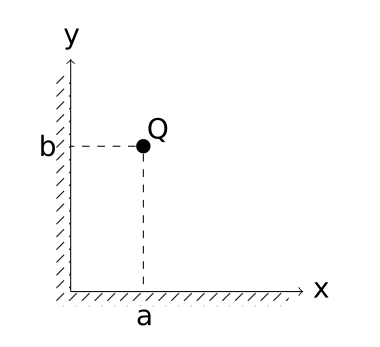
\includegraphics{media/Skizze.png}
    \label{fig:Spiegelladung}
   \end{figure}
\pagebreak
Aufgabe 3 : Kraftfeld
(5 Punkte)
Gegeben sei ein Kraftfeld
F ~ (~r ) =

a(3x − y)
b(2y − x)

mit a, b = const.
Ein punktförmiges Teilchen befinde sich in dem Kraftfeld F ~ (~r ). Berechnen Sie die Arbeit, die
beim Verschieben entlang der folgenden Wege geleistet wird:
 
t
(a) ~r 1 (t) =
mit t ∈ [0, 2]
t


t
(b) ~r 2 (t) =
mit t ∈ [0, 2]
t 2
2

(c) ~r 3 (t) =
2c cos(t)
3c sin(t)

mit t ∈ [0, 2π] und c = const.
(d) Ist die Kraft konservativ? Nennen Sie mindestens zwei Gründe für Ihre Antwort. Was
passiert für a = b?



Aufgabe 3: Delta-Distribution
(5 Punkte)
Die Delta Distribution kann durch
Z b
f ( x ) δ ( x ) dx = f ( 0 )
für
a < 0 < b
(6)
a
und
δ ( x ) = 0
für
x 6 = 0
(7)
definiert werden. Als Physiker*In dürfen Sie annehmen, dass δ sich wie eine „normale“
Funktion verhält und die üblichen Integrationsregeln gelten. Berechnen Sie
a) die Ableitung
Z b
f ( x ) δ 0 ( x ) dx (8)
f ( x ) δ ( cx − d ) dx (9)
f ( x ) δ ( g ( x )) dx (10)
a
b) eine Skalierung und Verschiebung
Z b
a
c) und die Verkettung mit g
Z b
a
von δ. Die Delts-Distribution kann auch als Grenzwert einer so genannten Dirac Folge
verstanden werden. Ein Beispiel für eine Diracfolge sind die Hammerschlag-Funktionen:
(
1
− 2 h < x < 2 h
A h ( t ) = h
(11)
0 sonst
d) Zeigen Sie, dass diese Folge für h → 0 gegen δ konvergiert.


Aufgabe 4:
Dielektrische Flüssigkeit im Zylinderkondensator
5 Punkte
Ein Zylinderkondensator bestehe aus zwei konzentrischen Röhren der Länge L = 1 m, wobei der
Abstand d = 1 mm zwischen den Röhren als klein gegen ihre Radien angenommen werden soll.
Nachdem der Kondensator mit einer Gleichspannungsquelle (U = 200 V) aufgeladen wurde, wird
das untere Ende des Kondensators in destilliertes Wasser knapp eingetaucht (Dichte ρ = 1 g/cm 3 ,
Dielektrizitätszahl ε = 81; Leitfähigkeit, kapillare Kräfte und Eintauchtiefe sind zu vernachlässi-
gen). Das Wasser steigt im Kondensator, wobei die zusätzliche Energie (potenzielle Energie des
Wassers und Feldenergie) von der Spannungsquelle geliefert wird.
Berechnen Sie die Höhe h der Wassersäule, die sich nach dem Einschwingen einstellt, indem Sie die
wirkenden Kräfte betrachten.


Sei M = [0, 1] 2 das Einheitsquadrat im R 2 und ~v : R 2 → R 2 das durch
~v (x, y) =
x + e −y 2
y + e −x 4
!
definierte Vektorfeld.
R
a) Stellen Sie ∂M ~v · ~n ds, wobei ~n der äußere Normalenvektor der Länge 1 von
∂M ist, als Summe von 4 gewöhnlichen Integralen dar und vereinfachen Sie
Ihr Ergebnis soweit wie möglich.
b) Berechnen Sie das Integral mit Hilfe des Satzes von Gauß.
